\documentclass{article}
\usepackage[UTF8]{ctex}
\usepackage{geometry}
\usepackage{multirow}
\usepackage{natbib}
\geometry{left=3.18cm,right=3.18cm,top=2.54cm,bottom=2.54cm}
\usepackage{graphicx}
\pagestyle{plain}	
\usepackage{setspace}
\usepackage{enumerate}
\usepackage{caption2}
\usepackage{datetime} %日期
\renewcommand{\today}{\number\year 年 \number\month 月 \number\day 日}
\renewcommand{\captionlabelfont}{\small}
\renewcommand{\captionfont}{\small}
\begin{document}

\begin{figure}
    \centering
    
\includegraphics[width=8cm]{upc.png}

    \label{figupc}
\end{figure}

	\begin{center}
		\quad \\
		\quad \\
		\heiti \fontsize{45}{17} \quad \quad \quad 
		\vskip 1.5cm
		\heiti \zihao{2} 《计算科学导论》个人职业规划
	\end{center}
	\vskip 2.0cm
		
	\begin{quotation}
% 	\begin{center}
		\doublespacing
		
        \zihao{4}\par\setlength\parindent{7em}
		\quad 

		学生姓名:\underline{\qquad  孙萃 \qquad \qquad}

		学\hspace{0.61cm} 号:\underline{\qquad 2007010219\qquad}
		
		专业班级:\underline{\qquad 计科2002 \qquad  }
		
        学\hspace{0.61cm} 院:\underline{计算机科学与技术学院}
% 	\end{center}
		\vskip 1.5cm
		\centering
		\begin{table}[h]
            \centering 
            \zihao{4}
            \begin{tabular}{|c|c|c|c|c|c|c|c|c|}
            % 这里的rl 与表格对应可以看到,姓名是r,右对齐的;学号是l,左对齐的;若想居中,使用c关键字。
                \hline
                \multicolumn{5}{|c|}{分项评价} &\multicolumn{2}{c|}{整体评价}  & 总    分 & 评 阅 教 师\\
                \hline
                自我 & 环境 & 职业 & 实施 & 评估与 & 完整性 & 可行性 &\multirow{2}*{} &\multirow{2}*{}\\
                分析& 分析& 定位 & 方案 & 调整 & 20\% & 20\% & ~&~ \\\            
                10\% & 10\% & 15\% & 15\% & 10\% & &  &~ &~\\
                \cline{1-7} 
                & & & & & & & ~&~ \\
                & & & & & & & ~&~ \\
                \hline      
            \end{tabular}
        \end{table}
		\vskip 2cm
		\today
	\end{quotation}

\thispagestyle{empty}
\newpage
\setcounter{page}{1}
% 在这之前是封面,在这之后是正文
      {目录}\par
	(一)	前言…………………………………………………………………………………………\par
	(二)	自我分析\par	
	a)	2.1自然条件…………………………………………………………………………\par
	b)	2.2.性格分析………………………………………………………………………\par
	c)  2.3.教育与学习经历………………………………………………………\par	
	d)	2.4.工作与社会阅历………………………………………………………\par
	e)  2.5知识、技能与经验……………………………………………………\par
	f)  2.6兴趣爱好与特长…………………………………………………………\par
	(三)	环境分析\par
	a)  3.1社会环境分析………………………………………………………………\par
	b)	3.2家庭环境分析………………………………………………………………\par
	c)	3.3职业环境分析………………………………………………………………\par
	d)	3.4地域与人际环境分析………………………………………………\par
	e)  3.5发展趋势…………………………………………………………………………\par
	(四)	职业定位\par	
	a)  4.1行业领域定位与理由………………………………………………\par
	b)  4.2职业岗位起点定位与理由……………………………………\par
	c)  4.3职业目标与可行性分析…………………………………………\par
	(五) 实施方案……………………………………………………………………………\par
	(六) 评估与调整………………………………………………………………………\par
	a)  6.1评估时间………………………………………………………………………\par
	b)  6.2评估内容……………………………………………………………………\par
	c)  6.3调整原则……………………………………………………………………\par	
	(七)	结束语………………………………………………………………………………\par
\section{前言}\par	
中国石油大学(华东)是石油、石化专业技术、管理(高层次)人才培养的重要基地,被誉为“石油、石化科技人才的摇篮”。经过半个世纪的建设和发展,该大学现已成为一所以工为主,多学科协调发展的大学。\par
一艘船,如果沿着明确的航程向前行驶,即使浓雾弥漫整个海面,即使狂风掀起奔腾的浪花,那么它也必将能到达彼岸的渡口。一个人,如果目光坚定旅途清晰,即使荆棘和坎坷布满道路,即使风雨和霜雪时时侵袭,那么他也必将能踏进成功的殿堂。因此,职业规划的必要性可想而知,下面我将据此完成一份职业生涯规划书。\par
\section{自我分析}
\par
\subsection{自然条件}
性别:男\par
年龄:18\par
身体条件:优秀\par
健康情况:健康\par
居住城市:家乡辽宁丹东,现于山东青岛深造\par
\subsection{性格分析}
优势:\par
	 1)  敢于冒险,敢于尝试新事物,能克服障碍\par
     2)	 兴趣广泛,对自己感兴趣的东西接受能力强\par
     3)	能统观全局、能看出行为和思想之间的潜在含义\par
     4)	交际能力强、能激发别人的热情\par
     5)	适应能力强,对新环境、新事物能迅速适应\par
     6)	能洞察别人,能理解他们的需要和动机\par
     7)  理解能力强,对陌生事物的可以通过表象渐渐了解本质\par
劣势:\par
	 1)不善于把握事物的轻重,难于决定优先处理哪些事\par
     2)对缺乏独创性的人没有耐心\par
     3)不愿以传统或常规的方式行事\par
     4)易于烦躁或不耐烦,尤其是当其作中创造性过程结束后\par
     5)讨厌做重复性任务\par
     6)不能容忍与过于严谨的机构或个人工作\par
	 7)倾向于关注可能发生的事情\par
\subsection{教育与学习经历}
目前就读于中国石油大学(华东),计算机科学与技术、本科。\par
计算机科学与技术专业知识体系:通识类知识、学科基础知识和专业知识。\par
相关课程:程序设计、数据结构、计算机组成、操作系统、计算机网络、信息管理,包括核心概念、基本原理以及相关的基本技术和方法\par
\subsection{工作与社会阅历}
曾以志愿者身份参加学生会工作;参加志愿服务活动,普及光盘行动意义,调查大众节约粮食意识;将于即将到来的寒假时间,进行回校宣讲,在宣传母校的同时,培养组织协调能力,语言表达能力。
\par
\subsection{知识、技能与经验}
1)组织能力:有过儿童节主持人的经验,并圆满完成任务;组织过各类团体活动,并有良好的反应;能够带领大家有序进行各项检查、活动。\par
2)指导能力:能在自己擅长的方面,积极主动指出他人缺点,并及时纠正指导,尽自己所能,跟他讲明白,学明白,改明白。\par
3)社交能力:能够很快的融入新的环境,结交新的朋友,并且相处融洽,能够在集体活动中,串联团队。
\par
\subsection{兴趣爱好与特长}
1)篮球:从小学接触篮球,曾在校队参加过比赛,并取得一定成绩,到如今参加院队,希望明年能取得好的成绩。\par
2)音乐:有一定音乐细胞,参加中国石油大学(华东)合唱团。对吉他有一定程度的学习,能够演奏简单的谱子\par
3)散打:跟随市散打队训练3年,能保护好自己和身边的人。
\par
\section{环境分析}
\subsection{社会环境分析}
中国政治稳定,经济持续发展。在全球经济一体化环境中的重要角色。经济发展有强劲的势头,加入wto后,会有大批的外国企业进入中国市场,中国的企业也将走出国门。目前社会对于计算机类人才需求高居不下,特别是我国的卡脖子问题不能得到解决的今天,具有一定能力的高水平毕业生一定会得到企业的青睐。就当下华为受到美国制裁,芯片问题无法解决,多家公司正在寻找有创新能力、攻坚克难能力的高水平人才。所以说无论是从专业层面来说还是国家层面来说,学好计算机专业知识,培养创新精神,不怕苦不怕累精神,都是现在社会所急需的。
\par
\subsection{家庭环境分析}
经济情况:普通工薪阶级\par
家人期望:父亲希望能成就一番大业,要么对国家对社会有贡献,要么对百姓对人民有责任;母亲相对佛系,以我的热爱为标准。\par
\subsection{职业环境分析}
(一)现状\par
随着互联网的发展,计算机专业人才的缺乏也没有得到有效缓解。国内的软件开发人才,网络技术、信息安全等方面的人才缺乏比较严重。那些高水平的系统分析师,资深项目策划人员非常少,能够解决中国科技卡脖子问题的真正的高水平人才供不应求,从事程序开发的程序员也比较缺乏。\par
(二)发展趋势\par
计算机专业近些年来一直是全国各大高校的热门专业,发展迅速。随着互联网的发展形势,计算机专业的人才将会短缺的非常严重,虽然每年的报考人数很多,但是高学历、高能力的计算机人才依旧稀缺。在国内,IT人才、电子商务人才、网络存储人才、游戏技术人才的严重短缺情况下在软件人才层次结构上,水平较高的系统分析员和有行业背景项目的策划人员偏少。\par
计算机应用技术专业人才市场需求量大,但中小学计算机教师需求量减少。随着计算机与网络应用的普及,计算机软件的大量使用,带动了相关产业的迅猛发展,急需大量专业的编程人员及项目负责人或相关工程师等专业人才。另外,随着电子商务的发展,计算机网络应用人才和网络安全人才显得非常缺乏。从人才需求调查表的结果看,计算机应用专业人才需求非常旺盛,优秀毕业生供不应求。\par
(三)就业方向\par
软件就业方向有软件开发,软件架构师,软件测试,应用软件 (包括手机程序 ) 的 调试、运行、测试、维护及质量管理等技术岗位的工作。 JAVA 软件开发,软件公司中 Java 软件工程师、网络工程师、数据库工程师等相关职位。\par
网络与信息安全方向宽口径专业,主干学科为信息安全和网络工程。学生毕业后可为政府、国防、军队、电信、电力、金融、铁路等部门的计算机网络系统和信息安全领域进行管理和服务的高级专业工程技术人才。\par
(四)发展前景\par
计算机技术专业在诸多方面就业前景都比较好,例如:\par
(1)网络工程方向就业前景良好,学生毕业后可以到国内外大型电信服务商、大型通信设备制造企业进行技术开发工作,也可以到其他企事业单位从事网络工程领域的设计、维护、教育培训等工作。\par
(2)软件工程方向 就业前景十分广阔,学生毕业后可以到国内外众多软件企业、国家机关以及各个大、中型企、事业单位的信息技术部门、教育部门等单位从事软件工程领域的技术开发、教学、科研及管理等工作。也可以继续攻读计算机科学与技术类专业研究生和软件工程硕士。\par
(3)通信方向学生毕业后可到信息产业、财政、金融、邮电、交通、国防、大专院校和科研机构从事通信技术和电子技术的科研、教学和工程技术工作。\par
(4)网络与信息安全方向宽口径专业,主干学科为信息安全和网络工程。学生毕业后可为政府、国防、军队、电信、电力、金融、铁路等部门的计算机网络系统和信息安全领域进行管理和服务的高级专业工程技术人才。并可继续攻读信息安全、通信、信息处理、计算机软件和其他相关学科的硕士学位。\par
\subsection{地域与人际环境分析}
目标城市:青岛、北上广深。\par
气候水土:青岛地处北温带季风区域,属温带季风气候。市区由于海洋环境的直接调节,受来自洋面上的东南季风及海流、水团的影响,故又具有显著的海洋性气候特点。空气湿润,雨量充沛,温度适中,四季分明。\par
\subsection{发展趋势}\par
至今,青岛连续十年入围宜居城市十强;

至今,青岛连续十年入围游客接待量十强;

至今,青岛连续十年入围出境游人数十强;

至今,青岛连续十年入围全国最佳治安城市十强;

至今,青岛连续十年入围应届研究生流入目的地十强。
\begin{figure}[h!]
	\centering
	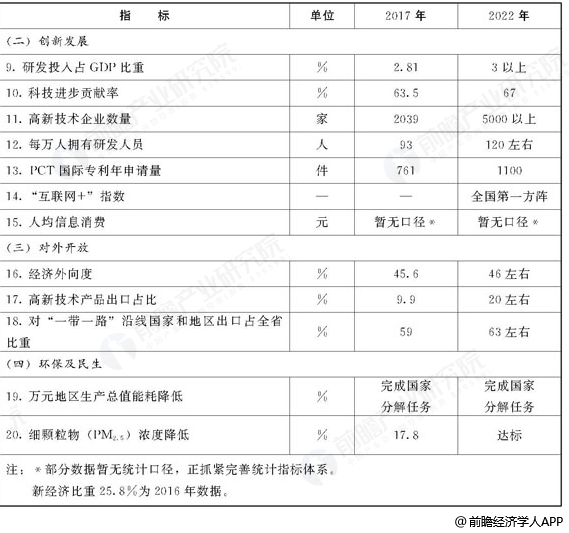
\includegraphics[scale=0.5]{1}
	\caption{The 1}
	\label{fig:1}
\end{figure}
\begin{figure}[h!]
	\centering
	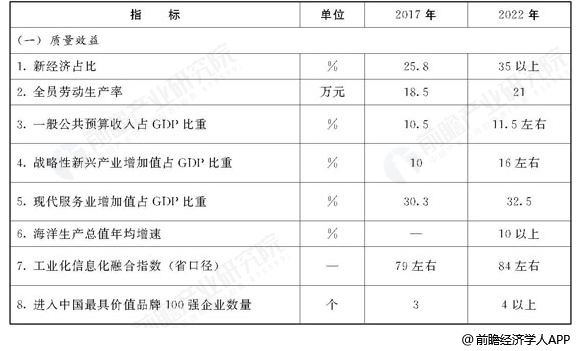
\includegraphics[scale=0.6]{2}
	\caption{The 2}
	\label{fig:2}
\end{figure}
\par
{\bf 总的来说,青岛前景光明,任重而道远}\par
\section{职业定位}
\subsection{行业领域定位与理由}
计算机科学与技术类专业毕业生的职业发展路线基本就两种:一种就是纯技术线路:信息产业属于朝阳产业,对人才提出了更高的要求,由于技术更新快,人才不得不不断补充新知识,对学习能力有着很高要求;另一种就是通过技术转型为管理,由技术型人才转型成为管理型人才。\par
在我深思熟虑之后,我觉得第二种由技术型人才转化成管理型人才更适合我,由于我性格更愿意去成为一名指挥家,所以我决定第二种路线。\par
就技术型方面,我想对应软件工程师的方向,从事软件开发,维护等领域。\par
就管理型方面,我想从事项目策划或者专业培训师或者系统经理,去计划指挥协调相关活动。\par
\subsection{职业岗位起点定位与理由}
计算机程序设计师,网络工程师,软件开发工程师,到达一定水平后架构师。\par
首先是兴趣驱动,我很希望有一天能够创造出属于自己的东西,喜欢创新,与众不同,不喜欢一成不变的东西,而且比较享受别人因为我的努力收益。\par
其次我认为要想以后能够成功转型成为管理型,我认为首先最必要的是在专业领域的能力要达到一定高度,要经历过相关领域的工作,懂得各个环节的困难点,易错点,为了以后能够能好的完成协调策划任务,认清任务重难点。\par	
\par
\subsection{职业目标与可行性分析}
(1)短期目标\par
\begin{itemize}
	\item 大一:学好公共基础课,为接下来的专业课打好基础,在课余时间参加ACM俱乐部,学习相关算法知识,在即将到来的寒假,自学python,html,了解计算机硬件,研究培养方案。\par
	公选课优先选择软件设计或管理类相关课程:例如多媒体应用基础,组织行为学,5g与通信工程。\par
	大一还是要好好学习,争取一下保研名额。\par
	\item 大二:选修python语言,加强英语词汇积累,听力练习,考取英语四级;继续跟随ACM俱乐部练习算法,参加一些算法比赛或者程序设计大赛,认识到差距,进一步学习进步。在暑假尝试开始实习,进入企业了解就业环境,了解所需技能,发现技能、知识的漏洞,回去恶补。(认真考虑行业发展,分析自身情况,确定是否要考研)\par
	
	\item 大三:选修管理类,金融类选修课,为后来人才转型打下基础。加强英语词汇积累,听力练习,写作能力,考取英语六级。在能力允许的情况下参加ACM竞赛,蓝桥杯,或者山东省大学生软件设计大赛。与同学组队,参加大创项目,争取一个好的名次。\par
	\item 大四:如果确定为就业的话:了解就业趋势,行业形势,为就业做好准备,了解各大企业招聘要求,学好自我介绍,培养应变能力,有一个好的心理素质,要保持自信。积极申请就业,参加招聘活动,在实践中发现不足,及时改进,听取前辈建议。\par
	如果确定要考研:就没什么可说的了,就应该全身心投入备考,尽所有所能,取得一个更高的成绩,去一个更高的平台。\par
\end{itemize}
\par
(2)中长期目标
\begin{itemize}
    \item 经济目标:1)在1年时,希望月薪5K~8K,能养活自己,并且有一点小额存款。\par
    			   2)在3~5年内,希望月薪1W~2W左右,有一定的存款,能够租一个环境相对好的房子。\par
    			   3)在5~10年,希望月薪有一个突破,然后就是不定上限吧,然后就希望能买一个自己的房子,风景好、交通方便就行。\par
    \item 能力目标:
    			  1)肯定是需要希望自己的研发能力,算法能力都有一个巨大的飞跃。\par
    			  2)管理能力有一个提升,尽量能达到系统架构师的一个最基本的要求。\par
    			  3)为人处世方面,情绪管理,能有一个进步。\par
    \item 职务目标:1)开发方向。2)能够成为项目经理,架构师。\par
\end{itemize}


\section{实施方案}
大一:探索期,首先要适应由高中生到大学生的角色转变,重新确定自己的学习目标和要求;其次,要开始接触职业和职业生涯的概念,特别要重点了解自己未来所希望从事的职业或与自己所学专业对口的职业,进行初步的职业生涯设计; 熟悉环境,建立新的人际关系,提高交际沟通能力,在职业 认识方面可以向高年级学生尤其是大四的毕业生询问就业 情况;积极参加各种各样的社团活动,增加交流技巧;在学习方面,要巩固扎实专业基础知识,加强英语、计算机能力的培养,掌握现代职业者所应具备的最基本技能;加强基础课的学习和编程语言的自我学习。\par
大二:认识自己的需要和兴趣,确定自己的价值观、 动机和抱负。考虑未来的毕业方向(深造或就业等),了解相关的活动,并以提高自身的基本素质为主,通过参加学生会或社团等组织,培养和锻炼自己的领导组织能力、团队协作精神,同时检验自己的知识技能;可以开始尝试兼职、社会实践活动,并要具有坚持性,最好能在课余时间从事与自己未来职业或本专业有关的工作,提高自己的责任感、主动性和受挫能力,并从不断的总结分析中得到职业的 经验;增加英语口语和计算机应用的能力,通过英语和计算机的相关证书考试,并开始有选择地辅修其他专业的知 识以充实自己。\par
大三:强专业知识学习的同时,考取与目标职业 有关的职业资格证书或相应地通过职业技能鉴定。因为临近毕业,所以目标应锁定在提高求职技能、搜集公司信息上。 参加与专业有关的暑期工作,和同学交流求职工作心得体会,学习写简历、求职信等求职技巧,了解搜集就业信息的渠道,如果有机会要积极尝试。\par
大四:这个阶段毕业方向已经确定,目标应该锁定在工作申请及成功就业上。这时,可先对前三年的准备做一个总结;首先检验自己已确立的职业目标是否明确,前三年的准备是否已充实;然后,开始毕业后工作的申请,积极参加招聘活动,在实践中检验自己的积累和准备;最后,进行预习或模拟面试。积极利用学校提 供的条件,了解就业指导中心提供的用人公司资料信息,强化求职技巧、进行模拟面试等训练,尽可能地在做好 较为充分的准备的情况下进行施展演练。在撰写毕业论 文的时,可大胆提自己的见解,锻炼自己独立解决问题的能 力和创造性。另外,要重视实习机会,通过实习从宏观上了 解单位的工作方式、运转模式、工作流程,从微观上明确个人在岗位上的职责要求及规范,为正式走上工作岗位奠定良好的基础。\par
\begin{enumerate}[1、]
	\item 利用交际能力,像更多的前辈学习;利用冒险精神,大胆尝试、创新;利用适应能力,尽快融入学习团队、工作团队,才能更好的进步。
	\item 弥补性格缺陷,在学习和工作上,能够更耐心、细心,尽量从重要性、紧急性,选择任务完成的顺序时间。
	\item 周围的人搞好关系,尽快融入团队。\par
		 积极工作,表现出吃苦耐劳的精神,在问题面前用于说出自己的看法,灵活应对各方考验,争取成为团队中有比较突出的表现。(既要在团体中展现自我,也要韬光养蓄)
	\item 
		注意从前辈那里学习相关的工作方法和技巧,每周对工作进行总结并形成书面或电子版保存下来。\par
		加强自己的收支管理。\par
		调节好自己的生活规律,按时锻炼,保持对篮球的热爱,保持健康的体魄。\par
		
\end{enumerate}
 依据以上自我探索,环境分析和职业定位,本人做出了以上实施计划。本实施计划的制定秉承着“意识 与性格的提升,学习与能力并重”的思想,只是在不同时期的侧重点有所不同。譬如本科阶段就以学习为重,能力的提升为辅。在这里学习与能力的提升和性格的完善是可以统一起来的,即在此过程中逐步完善自己的性格缺陷,将不适应自己职业发展的一些性格弱点如情感外露,容易急躁等逐步弱化以致完全克服。工作后是能力应用与意识提升阶段,即将以前获得的各种技能包括内在的心智上的发挥实际功用。这时学习岁仍然很重要,但已不是重点。重点是能力的应用和性格与意识的提升。意识的提升包括多个方面,比如对信息的把握和敏感度,是否始终有一颗进取心,对工作的热忱,自己看待事物所站的高度。一个人的职业意识决定了一个人的事业究竟能够做多大。当然上面所说的全是理论性的东西,是否能够指导一个人走向事业的顶峰还得看个人的素养与坚持。
\par 
\section{评估与调整}
由于影响职业生涯规划的因素很多,且大都处于动态变化之中,因此职业生涯规划应定期评估,并根据影响因素的变化和实施结果的情况及时作出调整,这样才能保证其行之有效。\par 
\subsection{评估时间}
每学期评估一次、每学年一次、三年评估一次。\par
\subsection{评估内容}
可以从成果目标、经济目标、能力目标、职务目标等方面总结,确定哪些目标已按预期实现,哪些目标商未达到,对已实现的成果总结经验,对未完成的目标分析原因。\par
每次评估之后根据规划书中,未实现、无法实现的目标进行及时的更改和反省,做出下一步的小的短期的目标,在大方向不变的情况下,尽可能完成。\par
\subsection{调整原则}
针对性原则——针对自身学习状况、家庭状况及所选职业发展状况\par
实事求是原则——如实评价自己各方面状况\par
特殊性原则——特殊情况应特殊对待\par
阶段性原则——根据自身状况对每个阶段计划做及时调整\par
完整性原则——计划的调整须照顾整个计划的完整性\par
\section{结束语}
任何目标,只说不做到头来都会是一场空。然而,现实是未知多变的,定出的目标计划随时都可能遭遇问题,因此要时刻报持有清醒的头脑。一个人,若要获得成功,必须拿出勇气,付出努力、拼搏、奋斗。\par
成功,不相信眼泪;未来,要靠自己去打拼!所谓“生命在于运动,人生在于折腾”,就是要让生活充满活力,让生命绚烂多彩,让人生在浮浮沉沉、风云变幻中绽放精彩。然而,实现目标的历程需要付出艰辛的汗水和不懈的追求,因而不要因挫折而畏缩不前,不要因失败而一蹶不振;要有屡败屡战的精神,要有越挫越勇的气魄;成功最终会属于你的,每天要对自己说:“ ’天生我材必有用’ ,我一定能成功,我一定按照目标的规划行动,坚持直到胜利的那一天。”既然选择了认准了是正确的,就要一直走下去。\par
未来还是未知的,现在的行动仅仅是个开始。我要迈出艰难的一步,朝着这个规划的目标前进,要以满腔的热情去获取最后的胜利。我的未来我做主,我的未来不是梦!\par
\end{document}
